%%
%% MOSAIC Bioinformatics manuscript
%% Donor-disjoint evidence closure, 2026-07-23.
%%
\documentclass[unnumsec,webpdf,contemporary,large,numbered]{oup-authoring-template}

\usepackage{booktabs}
\usepackage{array}
\usepackage{multirow}
\usepackage{graphicx}
\usepackage{xcolor}
\setlength{\emergencystretch}{2em}
\renewcommand{\dbltopfraction}{0.95}
\renewcommand{\dblfloatpagefraction}{0.85}
\setcounter{dbltopnumber}{2}

% OUP template v1.2 resets natbib to author-year mode for plain \bibitem
% entries, which renders numbered citations as empty brackets.
\makeatletter
\renewcommand\NAT@force@numbers{\global\NAT@numberstrue}
\makeatother

\begin{document}

\journaltitle{Bioinformatics}
\DOI{}
\copyrightyear{2026}
\pubyear{2026}
\vol{XX}
\issue{x}
\access{}
\appnotes{Original Paper}
\firstpage{1}

\title[MOSAIC]{MOSAIC: branch-supervised CITE-seq annotation with auditable modality evidence under donor shift and incomplete protein panels}

\author[1,2,$\dagger$]{Hai Yang}
\author[2,$\dagger$]{Linhao Wu}
\author[3,4]{Dan Zhou}
\author[5]{Tianyi Zhou}
\author[1,2]{Qin Zhou}
\author[1,2]{Ting Xiao}
\author[1,2]{Qian Zhang}
\author[1,2]{Jing Zhang}
\author[1,2,$\ast$]{Zhe Wang}

\address[1]{\orgdiv{Key Laboratory of Smart Manufacturing in Energy Chemical Process, Ministry of Education}, \orgname{East China University of Science and Technology}, \orgaddress{\postcode{200237}, \state{Shanghai}, \country{China}}}
\address[2]{\orgdiv{Department of Computer Science and Engineering}, \orgname{East China University of Science and Technology}, \orgaddress{\postcode{200237}, \state{Shanghai}, \country{China}}}
\address[3]{\orgdiv{Department of Big Data in Health Science}, \orgname{Zhejiang University School of Medicine}, \orgaddress{\state{Hangzhou}, \country{China}}}
\address[4]{\orgdiv{Center of Clinical Big Data and Analytics}, \orgname{The Second Affiliated Hospital, Zhejiang University School of Medicine}, \orgaddress{\state{Hangzhou}, \country{China}}}
\address[5]{\orgdiv{Department of Electrical Engineering and Computer Science}, \orgname{University of Michigan}, \orgaddress{\postcode{48109}, \state{Michigan}, \country{USA}}}

\corresp[$\ast$]{Corresponding author. \href{mailto:wangzhe@ecust.edu.cn}{wangzhe@ecust.edu.cn}}
\corresp[$\dagger$]{These authors contributed equally to this work.}

\received{Date}{0}{2026}
\revised{Date}{0}{2026}
\accepted{Date}{0}{2026}

\abstract{
\textbf{Motivation:} Fine-grained CITE-seq annotation is often reused across donors and antibody panels, but cell-level random splits can obscure donor shift, modality conflict and fragile sibling-state boundaries.\\
\textbf{Results:} We present MOSAIC, a branch-supervised RNA--ADT classifier that reports RNA-only, ADT-only and fused predictions, branch margins and bounded hierarchy-aware sibling refinement (HSR) actions. In nested leave-one-donor-out evaluation of 161,764 PBMCs and 58 labels, MOSAIC full reached ACC 0.9119 [0.9086, 0.9153], W-F1 0.9108 [0.9062, 0.9153] and M-F1 0.8072 [0.7917, 0.8227] across eight held-out donors. Relative to matched early fusion, paired donor differences were +0.0040 W-F1 [0.0013, 0.0066] and +0.0148 M-F1 [0.0091, 0.0206], whereas the ACC interval crossed zero. Branch disagreement detected errors with AUROC 0.755 [0.745, 0.766], above final-prediction uncertainty (0.691 [0.651, 0.732]), and branch top-two margins were positively associated with correctness (mean Spearman $\rho=0.378$). HSR changed 0.15\% of predictions and was same-checkpoint equivalent to disabling HSR within $\delta=0.005$. With 50\% proteins masked, W-F1 decreased by 0.0137. Validation-selected leave-class-out rejection achieved mean unknown recall 0.403 at observed known coverage 0.788, ranging from about 0.13 to 0.57 across targets; the hardest target lacked a matched light-chain ADT marker. On PDC101, the official marker-hierarchy method MMoCHi remained stronger.\\
\textbf{Availability and implementation:} Source code, split manifests, evidence tables and checksum records are described in the Code availability and Supplementary Material sections.\\
\textbf{Contact:} \href{mailto:wangzhe@ecust.edu.cn}{wangzhe@ecust.edu.cn}\\
\textbf{Supplementary information:} Supplementary material accompanies this manuscript.
}

\keywords{single-cell annotation, CITE-seq, multimodal learning, donor shift, missing modality, selective prediction, model auditing}
\keywords[Abbreviations]{ACC: accuracy; ADT: antibody-derived tag; AUPRC: area under the precision--recall curve; AUROC: area under the receiver operating characteristic curve; B-ACC: balanced accuracy; CI: confidence interval; CITE-seq: cellular indexing of transcriptomes and epitopes by sequencing; ECE: expected calibration error; HSR: hierarchy-aware sibling refinement; HTO: hash-tag oligonucleotide; KD: knowledge distillation; KL: Kullback--Leibler; LODO: leave-one-donor-out; M-F1: macro F1; MLP: multilayer perceptron; PBMC: peripheral blood mononuclear cell; PDC101: the GSE229791 sorted-holdout donor; TOST: two one-sided tests; W-F1: weighted F1}

\maketitle

\section{Introduction}

Single-cell RNA sequencing and CITE-seq jointly measure transcriptomic programs and surface-protein markers at cellular resolution \citep{hao2021,stoeckius2017cite,luecken2019}. RNA captures broad lineage and cell-state programs, whereas antibody-derived tags (ADTs) directly measure canonical surface markers. Integrated references now resolve fine immune populations, but supervised annotation remains difficult when labels separate closely related naive, central-memory, effector-memory, regulatory and activated states.

The practical value of an annotation model is therefore determined by more than average accuracy on a convenient held-out cell set. Target cohorts often differ in donor composition, antibody panel or disease state, and a classifier may still output a confident fine label after the relevant sibling boundary has shifted. A useful model should make this distinction visible by reporting the fine label, modality evidence, confidence and conservative parent-level fallback when needed.

Most annotation benchmarks still emphasize cell-level random splits. Such splits can place cells from the same donor in training and test, leading performance to combine annotation ability with donor-specific reuse. In practical reuse, the reference and target studies may differ in donor composition, antibody panel, disease status and missing cell states. A model that performs well under a random split can therefore fail silently when the protein panel changes, when only RNA is available, or when a target population was absent from the reference. Aggregate accuracy also hides rare-class errors and gives little indication of which modality or feature supported a decision.

Reference classifiers and semi-supervised systems include SingleR \citep{aran2019}, CellTypist \citep{dominguezconde2022}, scmap \citep{kiselev2018scmap}, scPred \citep{alquicira2020scpred}, scClassify \citep{lin2020scclassify} and scNym \citep{kimmel2021scnym}. scVI, scANVI and totalVI provide probabilistic representation learning and multimodal integration \citep{lopez2018,gayoso2022scvi,gayoso2021totalvi}. Benchmark rankings vary with task, modality and preprocessing, and methods such as MMoCHi show that a curated hierarchy can be strong when the panel and label space match the task \citep{caron2025mmochi}. These methods motivate evaluation that distinguishes predictive performance, robustness and biological interpretability rather than relying on a single headline score.

Existing methods cover many parts of this landscape, but they are rarely evaluated under a single audit protocol that simultaneously addresses donor-disjoint performance, incomplete protein input, leave-class-out behavior and quantitative interpretability. RNA-only label transfer is broadly applicable but cannot use ADT evidence when surface proteins define a boundary; multimodal generative models are often evaluated only as final-label predictors; and marker-rule systems can be highly accurate when hierarchy and panel are matched but less informative about learned classifiers under panel mismatch. We therefore ask a narrower question: whether an auditable RNA--ADT classifier can improve fine-level donor generalization over a matched neural baseline while reporting where that improvement does and does not hold.

We introduce MOSAIC, a compact dual-modal classifier designed to expose its prediction path. By auditable we mean that each prediction can be accompanied by per-modality labels and margins, the applied fusion policy, any bounded HSR action and the ranked RNA and ADT features stored in checksum-indexed artifacts. RNA, ADT and fused representations receive separate supervision; a training-only teacher supplies soft targets; branch logits are combined using top-two margins; and an HSR head can modify only prespecified local labels. Attention and sparse-expert models motivate modular prediction paths \citep{vaswani2017,shazeer2017moe}, but MOSAIC uses compact multilayer perceptrons to separate interface design from backbone scale.

This article makes four contributions. First, it evaluates RNA--ADT annotation with nested donor-disjoint splits, train-only preprocessing and donors as the statistical unit. Second, it defines a branch-supervised classifier interface that reports RNA-only, ADT-only and fused predictions from one checkpoint and yields usable error-detection signals. Third, it implements a bounded local HSR mechanism whose actions are restricted to declared sibling labels and can therefore be enumerated even when aggregate ablations are negative. Fourth, it reports method boundaries directly, including target-dependent rejection failure and a negative comparison with MMoCHi on its native sorted hierarchy.

The study asks four linked questions. First, does the model generalize to held-out donors under train-only preprocessing? Second, how does a frozen checkpoint degrade under protein-panel mismatch or RNA-only input? Third, can validation-selected rejection and parent fallback reduce leave-class-out failure? Fourth, are feature attributions stable across donors and enriched for prespecified markers? We also compare directly with official MMoCHi on its compatible PDC101 sorted holdout.

\section{Materials and methods}

\begin{figure*}[!t]
\centering
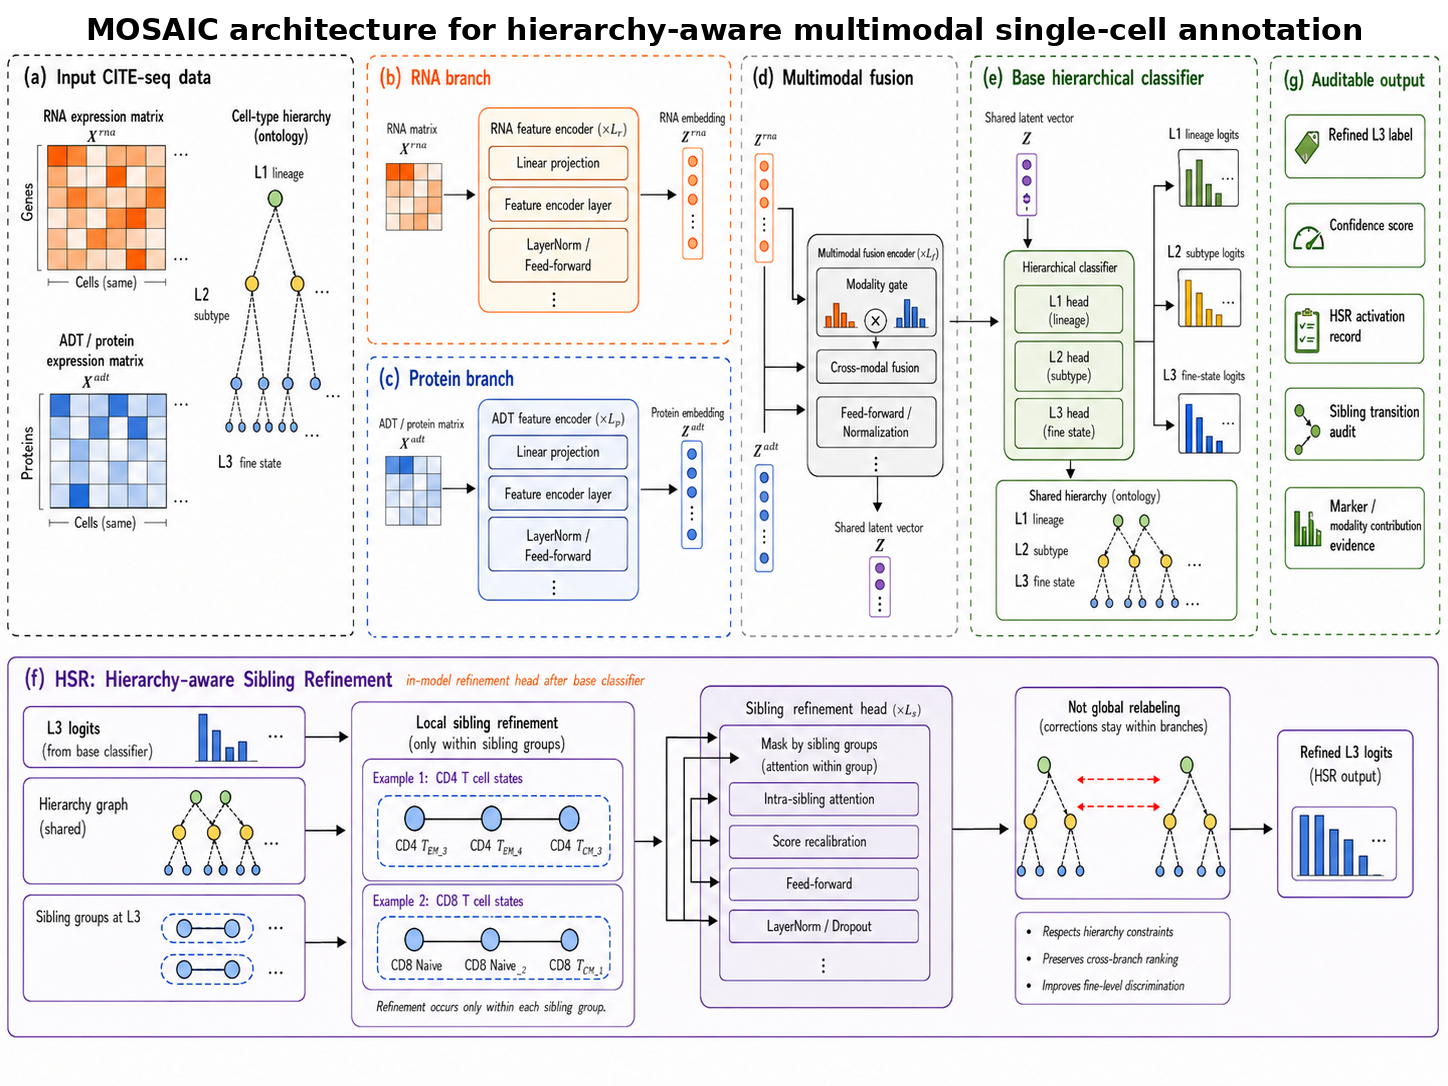
\includegraphics[width=\textwidth]{Fig/fig1_user_final.png}
\caption{\textbf{MOSAIC architecture.} (a) Paired CITE-seq RNA and ADT matrices and the cell-type hierarchy. (b,c) RNA and protein branches encode modality-specific representations. (d) Multimodal fusion combines both embeddings into a shared representation. (e) The base hierarchical classifier produces lineage, subtype and fine-state outputs. (f) Hierarchy-aware sibling refinement restricts local changes to prespecified sibling groups before producing refined L3 logits. (g) Auditable outputs summarize the refined label, confidence, HSR activity, sibling transitions and modality or marker evidence.}
\label{fig:architecture}
\end{figure*}

\subsection{Notation}

Let $N$ be the number of cells, $G$ the number of selected RNA genes, $P$ the number of ADT features and $C=58$ the number of L3 labels in the primary PBMC task. For cell $i$, $\mathbf{x}^{(r)}_i\in\mathbb{R}^{G}$ and $\mathbf{x}^{(p)}_i\in\mathbb{R}^{P}$ denote RNA and ADT input vectors. Encoders $f_r$, $f_p$ and $f_f$ produce RNA, ADT and fused embeddings $\mathbf{h}_r$, $\mathbf{h}_p$ and $\mathbf{h}_f$. Branch logits are $\mathbf{z}_r,\mathbf{z}_p,\mathbf{z}_f\in\mathbb{R}^{C}$, and $\mathbf{z}^{\mathrm{base}}$ denotes the margin-fused base logits before HSR. The teacher distribution is $\mathbf{q}$, and $\mathbf{p}^{T}=\operatorname{softmax}(\mathbf{z}^{\mathrm{base}}/T)$ is the student distribution at distillation temperature $T$. The HSR correction $\Delta\mathbf{z}\in\mathbb{R}^{C}$ is masked so that entries outside the declared sibling labels are exactly zero. The function $\sigma(\cdot)$ denotes the logistic sigmoid. To avoid conflict with loss symbols, encoder depth is referred to as $n_r$, $n_p$ and $n_f$ rather than $L_r$, $L_p$ and $L_f$.

\subsection{Datasets and donor-disjoint evaluation}

The primary dataset is the paired PBMC 3P cohort from GSE164378 \citep{hao2021}. It contains 161,764 cells from eight donors, 224 proteins and 58 fine-grained L3 labels. We used nested leave-one-donor-out evaluation. For test donor P1--P8, the validation donor was fixed as the next donor in a cycle (P1$\rightarrow$P2, \ldots, P8$\rightarrow$P1), and the remaining six donors formed training. Test sets ranged from 14,660 to 26,250 cells. All eight training folds contained all 58 labels, so the natural donor experiment tests donor shift under a closed-set label space.

Cells were partitioned before preprocessing. RNA values were log-transformed, 3,000 genes were selected from training donors, and RNA and ADT values were standardized with training-donor means and variances before applying the same transformations to validation and test cells. No CLR or DSB protein normalization was fitted inside the nested protocol. Model checkpoints, training hyperparameters and rejection thresholds were selected without test labels. The eight held-out donors, not cells or model seeds, are the biological replicates for the primary statistical comparison.

We used the L3 annotation level as the main endpoint because it is the level at which closely related immune states are most likely to be confused and at which a hierarchy-aware correction module is meaningful. The L1 and L2 hierarchy was retained for parent fallback and interpretation, but not used to inflate the primary closed-set score. Class imbalance was handled through sqrt-balanced training loss and macro-level reporting rather than through downsampling the test donors. This choice preserves the natural donor composition and makes W-F1, M-F1 and per-class F1 complementary: W-F1 reflects cohort-scale annotation quality, M-F1 reflects rare-label behavior and per-class F1 localizes sibling-level failures.

For a hierarchy-aware external comparator, we used the GSE229791 PDC101 sorted holdout with the official MMoCHi hierarchy and \texttt{external\_holdout=True} \citep{caron2025mmochi}. Hash-tag oligonucleotide (HTO), isotype and control proteins were excluded because PDC101 sort labels are linked to HTO/source information. MOSAIC used the identical 2,098-cell holdout and the same processed RNA/ADT input scale; scalers were fitted on training cells only. This comparison is compatible at the holdout and label-hierarchy level, but it is not pooled with the PBMC donor analysis because the sorted PDC101 task has a different label space and uncertainty mode.

Secondary COVID-19, 5P and COMBAT/COVID-shift artifacts were retained only as breadth evidence. The primary inference was restricted to the PBMC nested donor protocol and compatible PDC101 comparison, avoiding a heterogeneous leaderboard that mixes split units, label granularities and uncertainty estimates.

\subsection{MOSAIC model architecture}

For cell $i$, RNA and ADT inputs are $\mathbf{x}^{(r)}_i$ and $\mathbf{x}^{(p)}_i$. Modality encoders produce $\mathbf{h}_{r}=f_r(\mathbf{x}^{(r)})$ and $\mathbf{h}_{p}=f_p(\mathbf{x}^{(p)})$, and a fusion encoder maps their concatenation to $\mathbf{h}_{f}=f_f([\mathbf{h}_{r};\mathbf{h}_{p}])$. The primary configuration uses one hidden layer per encoder, hidden dimension 256, ReLU activation, dropout 0.2 and linear L3 heads for $\mathbf{z}_{r}$, $\mathbf{z}_{p}$ and $\mathbf{z}_{f}$. Separate cross-entropy losses keep the modality branches predictive, so the model can report RNA-only, ADT-only and fused predictions from the same checkpoint.

The arbitration signal for branch $b$ is its top-two logit margin $m_b=z_b^{(1)}-z_b^{(2)}$. Learned branch bias $\beta_b$ and temperature $\tau$ define
\begin{equation}
w_b=\operatorname{softmax}_b((m_b+\beta_b)/\tau),\qquad
\mathbf{z}^{\mathrm{base}}=\sum_{b\in\{r,p,f\}}w_b\mathbf{z}_b.
\end{equation}
The implementation learns $\beta_b$ and a shared $\tau$ during training and averages logits rather than probabilities, treating margins as ordering signals rather than calibrated branch-correctness probabilities.

HSR receives the fused embedding and detached base probabilities. A delta head predicts local corrections only for two fixed sibling groups: CD4 TEM\_3/CD4 TEM\_4/CD4 TCM\_3 and CD8 Naive/CD8 Naive\_2/CD8 TCM\_1. A bounded gate produces
\begin{equation}
\begin{aligned}
g &=0.02+0.18\,\sigma(\operatorname{MLP}([\mathbf{h}_{f};
\operatorname{stopgrad}(\operatorname{softmax}(\mathbf{z}^{\mathrm{base}}))])),\\
\mathbf{z}^{\mathrm{final}}&=\mathbf{z}^{\mathrm{base}}+g\,\Delta\mathbf{z}.
\end{aligned}
\end{equation}
All correction entries outside the six declared labels are set to zero by a fixed mask. The gate range $[0.02,0.20]$ was fixed as a conservative validation-time design choice; every activation can be counted, and negative HSR ablations indicate only that this bounded mechanism is insufficient, not that hierarchy information is useless in general.

\subsection{Training and statistical analysis}

Each donor fold used seeds 41, 42 and 43. An early-fusion MLP served as the matched baseline because it has the same RNA--ADT feature access without branch arbitration or HSR. The seed-42 MLP supplied stored training-cell probabilities to MOSAIC; validation and test teacher probabilities were never training inputs. This teacher is weaker than the final MOSAIC model and is used as a regularizing soft-label source rather than as a superior teacher. Because all MOSAIC seeds used the same seed-42 teacher within each fold, seed variation is not treated as an independent biological replicate. We retrained MLP, MOSAIC full, MOSAIC without HSR and MOSAIC without KD, and evaluated full checkpoints without retraining as RNA branch, ADT branch, fusion branch, uniform fusion, learned margin gate and learned margin gate plus HSR. Thus retrained ablations test training-time modules, whereas same-checkpoint ablations isolate inference-time arbitration and HSR.

The released default configuration is the locked MOSAIC full inference path, including learned margin arbitration and bounded HSR, because it is the configuration for which branch margins, arbitration weights and HSR actions are jointly audited. Uniform fusion is reported as a same-checkpoint sensitivity analysis and was not selected post hoc as the default after seeing test metrics.

The implemented objective combines sqrt-balanced cross-entropy, branch supervision, temperature-scaled KL distillation and the local HSR loss:
\begin{equation}
\mathcal{L}=\mathcal{L}_{\mathrm{wCE}}+
\lambda_b(\mathcal{L}^{\mathrm{CE}}_{r}+\mathcal{L}^{\mathrm{CE}}_{p})+
\lambda_f\mathcal{L}^{\mathrm{CE}}_{f}+
\lambda_{\mathrm{KD}}T^2D_{\mathrm{KL}}(\mathbf{q}\Vert\mathbf{p}^{T})+
\lambda_{\mathrm{HSR}}\mathcal{L}_{\mathrm{HSR}}.
\end{equation}
For class $c$ with training count $n_c$, the sqrt-balanced weight is proportional to $1/\sqrt{n_c}$ and normalized to have mean one across classes. $\mathcal{L}_{\mathrm{wCE}}$ is the weighted cross-entropy on $\mathbf{z}^{\mathrm{final}}$; $\mathcal{L}^{\mathrm{CE}}_r$, $\mathcal{L}^{\mathrm{CE}}_p$ and $\mathcal{L}^{\mathrm{CE}}_f$ are unweighted branch cross-entropies; and $\mathcal{L}_{\mathrm{HSR}}$ is the cross-entropy restricted to cells whose true label belongs to one of the declared sibling groups. The $T^2$ factor follows the standard temperature-scaled knowledge-distillation convention \citep{hinton2015distilling}. Models used AdamW for at most 35 epochs, batch size 1,024, learning rate $10^{-3}$, weight decay $10^{-4}$, dropout 0.2 and patience 14. We set $\lambda_b=0.35$, $\lambda_f=0.50$, $\lambda_{\mathrm{KD}}=0.05$, $T=2$ and $\lambda_{\mathrm{HSR}}=0.20$ before test evaluation. Checkpoints maximized validation M-F1 subject to validation ACC and W-F1 being within 0.0015 of their best observed values.

We report ACC, W-F1, M-F1, balanced accuracy and per-class F1. M-F1 was treated as the primary aggregate endpoint because it is most sensitive to rare sibling labels; ACC and W-F1 were secondary aggregate endpoints. Seeds were averaged within each held-out donor; donor means, 95\% Student-$t$ intervals, paired-difference intervals and Wilcoxon sensitivity tests were then calculated across eight donors. With $n=8$, a two-sided Wilcoxon value of 0.0078 corresponds to all donor differences sharing the same sign, so effect magnitudes are reported through paired intervals rather than through $P$ values alone. No cell-level bootstrap was used for the primary PBMC comparison. Exploratory attribution enrichment tests are reported as unadjusted marker-set checks and are not used as family-wise confirmatory claims.

All metrics were computed from frozen predictions generated before manuscript table construction. Table scripts consume prediction-level artifacts or summary CSV files and fail when a required metric is missing. PDC101 uncertainty estimates are not pooled because MOSAIC uses repeated seeds and MMoCHi uses a bootstrap of one official workflow.

\subsection{Robustness, rejection and interpretability analysis}

Each of the 24 full checkpoints was frozen and evaluated with full input; deterministic masks removing 10, 30, 50 or 70\% of proteins; prespecified memory-marker and T-cell-marker masks; and RNA-only input. Masks were fixed before test evaluation. These are stress tests of a full-input model under panel mismatch, not mask-aware training experiments.

Because every natural donor fold retained all 58 labels in training, unknown-label evidence used five prespecified leave-class-out targets: gdT\_2, NK\_3, CD4 TCM\_1, CD8 TEM\_4 and B naive lambda. Each model was retrained on 57 labels. Thresholds for one minus maximum probability, one minus top-two margin and energy were selected using known validation cells to target 0.95 or 0.80 known coverage. Known coverage is the fraction of known-label cells accepted for L3 output; unknown recall is the fraction of removed-label cells rejected; parent-safe rate is the fraction of rejected unknown cells whose predicted parent label is correct; and combined hierarchical accuracy counts accepted cells by L3 correctness and rejected cells by parent correctness. These scores are related to confidence calibration, uncertainty estimation and selective prediction \citep{guo2017calibration,lakshminarayanan2017,gal2016,hendrycks2017,geifman2017}.

Gradient-times-input attribution was computed for up to 64 correctly predicted cells per donor, seed and sibling label, with RNA and ADT summarized separately. We quantified donor-pair Spearman correlation, top-20 Jaccard overlap and canonical-marker enrichment using prespecified class--modality marker sets and 5,000 permutations. Deletion lift is the reduction in target probability after deleting top-ranked attribution features minus the matched reduction after deleting random features. Integrated gradients checked directional agreement on a small subset \citep{sundararajan2017}.

\subsection{Software implementation and reproducibility}

The Python/PyTorch implementation saves configuration, split manifest, selected checkpoint, predictions, per-class metrics, run log and SHA-256 artifact index for every training unit. Table and figure scripts consume declared CSV/JSON artifacts and reject incomplete matrices, so every reported row is traceable to a declared run rather than manually copied from logs.

The manuscript package contains table fragments, figure manifests, split definitions and audit scripts; raw data, caches and checkpoints are excluded but source accessions and checksum-indexed derived artifacts are recorded. Experiments used one NVIDIA RTX 4090. MOSAIC full had 2.51M trainable parameters and a median runtime of 130.0 seconds per fold--seed unit; the matched MLP had 1.73M parameters and a median runtime of 62.3 seconds (Supplementary Table S12).

\section{Results}

\subsection{Donor-disjoint annotation performance}

The first analysis asks whether the proposed workflow improves annotation when the test donor is absent from all preprocessing and training steps. Across eight held-out donors, MOSAIC full reached ACC 0.9119 (95\% CI 0.9086--0.9153), W-F1 0.9108 (0.9062--0.9153) and M-F1 0.8072 (0.7917--0.8227; Table~\ref{tab:donor-performance}; Fig.~\ref{fig:evidence}a). Relative to matched MLP, paired donor differences were $+0.0029$ ACC (CI $-0.0001$ to 0.0059), $+0.0040$ W-F1 (0.0013--0.0066) and $+0.0148$ M-F1 (0.0091--0.0206). Seven of eight donors improved in W-F1, and all eight improved in M-F1. The ACC interval crossed zero and is not claimed as significant.

This pattern is consistent with a rare-class and class-balance benefit rather than a broad increase in every cell-level decision; donor-paired W-F1 and M-F1 are therefore the main positive performance evidence.

To remove the training-cap caveat from the comparator matrix, we reran one published single-cell annotation package baseline and 12 classical or tree-based baselines using all available training donor cells in each fold and the complete held-out donor as test. The displayed ranking table contains CellTypist, XGBoost, ridge and centroid methods; Gaussian naive Bayes runs are retained as diagnostic artifacts but excluded from the ranking table because their high-dimensional likelihood assumptions produced clearly unstable rows. The published RNA-only CellTypist baseline reached ACC 0.8624, W-F1 0.8525 and M-F1 0.6357. The strongest added comparator remained early-fusion XGBoost, with ACC 0.9097, W-F1 0.9078 and M-F1 0.8017 across eight held-out donors (Supplementary Table S13). MOSAIC full had higher point estimates, but paired donor intervals versus XGBoost crossed zero: $+0.0023$ ACC (CI $-0.0085$ to 0.0131), $+0.0029$ W-F1 ($-0.0070$ to 0.0128) and $+0.0055$ M-F1 ($-0.0072$ to 0.0182; Supplementary Table S14). RNA-only scmap and scPred were retained only as additional tool-coverage artifacts because their local R/Bioconductor reproductions required method-specific tractability caps; they are not used as uncapped main-table comparators.

\begin{table*}[t]
\centering
\caption{Primary nested leave-one-donor-out PBMC 3P performance. Values are donor means with two-sided 95\% Student-$t$ confidence intervals after averaging seeds within each held-out donor ($n=8$ donors). Bold indicates the best value within each metric. MOSAIC full versus MLP paired donor differences were significant for W-F1 ($P=0.0101$) and M-F1 ($P=0.0005$), but not ACC ($P=0.0588$).}
\label{tab:donor-performance}
\scriptsize
\setlength{\tabcolsep}{3.2pt}
\renewcommand{\arraystretch}{0.95}
\resizebox{\textwidth}{!}{%
\begin{tabular}{lcccc}
\toprule
Metric & MLP early fusion & MOSAIC full & MOSAIC without HSR & MOSAIC without KD \\
\midrule
ACC & 0.9091 [0.9048, 0.9133] & 0.9119 [0.9086, 0.9153] & \textbf{0.9135 [0.9102, 0.9168]} & 0.9134 [0.9102, 0.9167] \\
W-F1 & 0.9068 [0.9020, 0.9116] & 0.9108 [0.9062, 0.9153] & 0.9121 [0.9079, 0.9162] & \textbf{0.9121 [0.9078, 0.9164]} \\
M-F1 & 0.7923 [0.7758, 0.8089] & 0.8072 [0.7917, 0.8227] & 0.8097 [0.7950, 0.8243] & \textbf{0.8110 [0.7956, 0.8265]} \\
Balanced accuracy & 0.7796 [0.7629, 0.7964] & \textbf{0.8085 [0.7890, 0.8280]} & 0.8067 [0.7895, 0.8238] & 0.8079 [0.7913, 0.8244] \\
\bottomrule
\end{tabular}

}
\end{table*}

\subsection{Ablation analysis of MOSAIC components}

Direct ablations did not identify HSR, KD or learned margin arbitration as sources of the aggregate improvement over MLP. Retrained no-HSR exceeded full by 0.0016 ACC and 0.0025 M-F1; no-KD exceeded full by 0.0015 ACC and 0.0038 M-F1. Within the same full checkpoints, uniform fusion exceeded learned margin gate plus HSR on all eight donors by 0.0011 ACC, 0.0011 W-F1 and 0.0042 M-F1. Enabling HSR within the same checkpoint changed aggregate metrics by less than 0.0005 and produced mixed directions.

These negative results delimit the architecture. The branch-supervised model is useful as an auditable multimodal classifier, but this experiment does not prove that bounded HSR or learned gating drives the donor-level gain. The default full configuration is retained for auditability rather than because it maximizes every aggregate metric; users focused only on closed-set aggregate accuracy can inspect the reported uniform-fusion sensitivity result. HSR and margin gating remain software and workflow contributions because they expose whether a local sibling correction was available, whether it fired and which labels were affected.

We additionally ran a branch-loss sensitivity matrix under the same nested donor protocol (Fig.~\ref{fig:evidence}b). Removing branch supervision while keeping the three-branch architecture gave ACC 0.9102 and M-F1 0.8084; a stronger branch weight $\lambda_b=0.70$ gave the highest ACC and W-F1 (0.9140 and 0.9126), whereas late-fusion-only training gave the highest M-F1 and balanced accuracy (0.8122 and 0.8132; Supplementary Table S3). Branch supervision changes the accuracy--macro balance and enables branch-level evidence, but it is not a monotonic universal performance driver.

To quantify auditability, we tested whether branch disagreement predicts errors (Fig.~\ref{fig:evidence}c). The three-branch vote-disagreement score, defined as whether branch top labels disagree, achieved donor-level error-detection AUROC 0.7552 (95\% CI 0.7445--0.7659), compared with 0.6914 (0.6507--0.7320) for final prediction uncertainty. Its AUPRC and 90\% coverage risk were not better than uncertainty, so we interpret branch disagreement as a complementary audit signal rather than a replacement for confidence-based selection. A branch margin-correctness audit further showed that top-two logit margins positively ordered branch correctness (Fig.~\ref{fig:evidence}d): mean Spearman correlation was 0.3777 (0.3653--0.3900) across branches, and top-quintile branch accuracy exceeded bottom-quintile accuracy by 0.3705 (0.3641--0.3768; Supplementary Table S5). HSR action auditing showed a prediction-change rate of only 0.0015 (0.0010--0.0020), with wrong-to-correct and correct-to-wrong rates both approximately 0.0006; TOST supported HSR same-checkpoint equivalence within the prespecified $\delta=0.005$ equivalence margin \citep{lakens2017} for all four aggregate metrics (Supplementary Table S4). The remaining architecture claim is therefore narrow: MOSAIC exposes branch and local-refinement evidence while matching or improving donor-level macro behavior relative to early fusion.

\subsection{Robustness to incomplete protein panels}

At 50\% random protein masking, W-F1 was 0.8971, a donor-level decrease of 0.0137 from full input; at 70\% masking it was 0.8921 (Fig.~\ref{fig:evidence}e). RNA-only input reached W-F1 0.8882, a decrease of 0.0226. M-F1 was more sensitive, decreasing by 0.0330 at 50\% masking and 0.0514 for RNA-only input. ECE increased from 0.0713 to 0.1063 for RNA-only input.

The result shows gradual degradation rather than abrupt collapse, but rare labels and calibration were more fragile than W-F1 and marker-group masks can be more damaging than random masks. Because full input remained strongest, masking is treated as a deployment audit rather than a solved robustness problem.

\subsection{Hierarchical rejection under leave-class-out stress tests}

At target known coverage 0.80, one-minus-margin rejection achieved observed known coverage 0.7878, mean unknown recall 0.4032 and combined hierarchical accuracy 0.9146 (Supplementary Tables S7--S8). Energy gave similar recall (0.4024) but lower combined hierarchical accuracy (0.9073). Results varied sharply by target: mean margin-based recall was approximately 0.57 for CD4 TCM\_1 and gdT\_2 but 0.13 for B naive lambda. Unknown parent-safe rate was 0.2259 overall.

The leave-class-out experiment forces the model to classify cells whose fine label was removed from the reference, with rejection thresholds selected only from known validation cells. The target dependence, especially low recall for B naive lambda, shows that confidence scores support selective prediction and parent fallback for some labels but not general open-world recognition.

\subsection{External hierarchy baseline and attribution stability}

On the PDC101 holdout, MOSAIC achieved 0.9077 ACC, 0.9068 W-F1 and 0.9007 M-F1, while official MMoCHi achieved 0.9347, 0.9335 and 0.9298 (Supplementary Tables S10--S11). The uncertainty modes differ: MOSAIC uses three-seed Student-$t$ margins, whereas MMoCHi uses a cell bootstrap conditional on one workflow fit. The result establishes a compatible direct comparison and a negative method boundary. It also clarifies the task distinction: a curated hierarchy with marker-aware rules can be stronger in a small sorted label space, whereas MOSAIC is designed for high-dimensional reference-trained annotation and auditability under donor and modality stress tests.

Across donor pairs, mean attribution Spearman correlation ranged from 0.529 to 0.796 for RNA and from 0.295 to 0.612 for ADT (Supplementary Table S15). Ten of 12 class--modality tests showed canonical-marker enrichment at unadjusted permutation $P<0.05$. CD4 TEM\_4 ADT and CD8 Naive RNA did not. These marker-enrichment tests are exploratory because the donor-pair summaries overlap and no family-wise biological-discovery claim is made. Seed-level attribution stability and integrated-gradient checks were generally stronger than donor-pair overlap, indicating that donor variation, not only model initialization, limits interpretation. The attribution analysis is therefore quantitative evidence of reproducibility and marker concordance for selected sibling classes.

The attribution evidence connects the model to biological review criteria by testing reproducibility and marker enrichment rather than relying on selected heatmaps. We added a perturbation check in which top attribution features were zeroed and compared with matched random features. Top-feature deletion reduced target probabilities more than random deletion in all six ADT tests and all six RNA tests, with mean deletion lifts of 0.2358 for ADT and 0.1304 for RNA (Fig.~\ref{fig:evidence}f; Supplementary Table S4). This supports attribution faithfulness for the selected sibling classes. The B naive lambda leave-class-out failure is also biologically interpretable: IGKC, IGLC2 and IGLC3 were retained in every donor fold, but the ADT panel contained no kappa/lambda surface marker (Supplementary Table S9; Supplementary Fig. S1a). Thus the difficult unknown target is not simply a model-confidence artifact; it reflects a sparse marker-defined boundary with incomplete protein evidence. Conversely, PDC101 shows a boundary where a curated marker hierarchy remains stronger: the largest MMoCHi advantages occur for CD8 central-memory/effector-memory-related labels, not monocytes (Supplementary Fig. S1b).

\begin{figure*}[t]
\centering
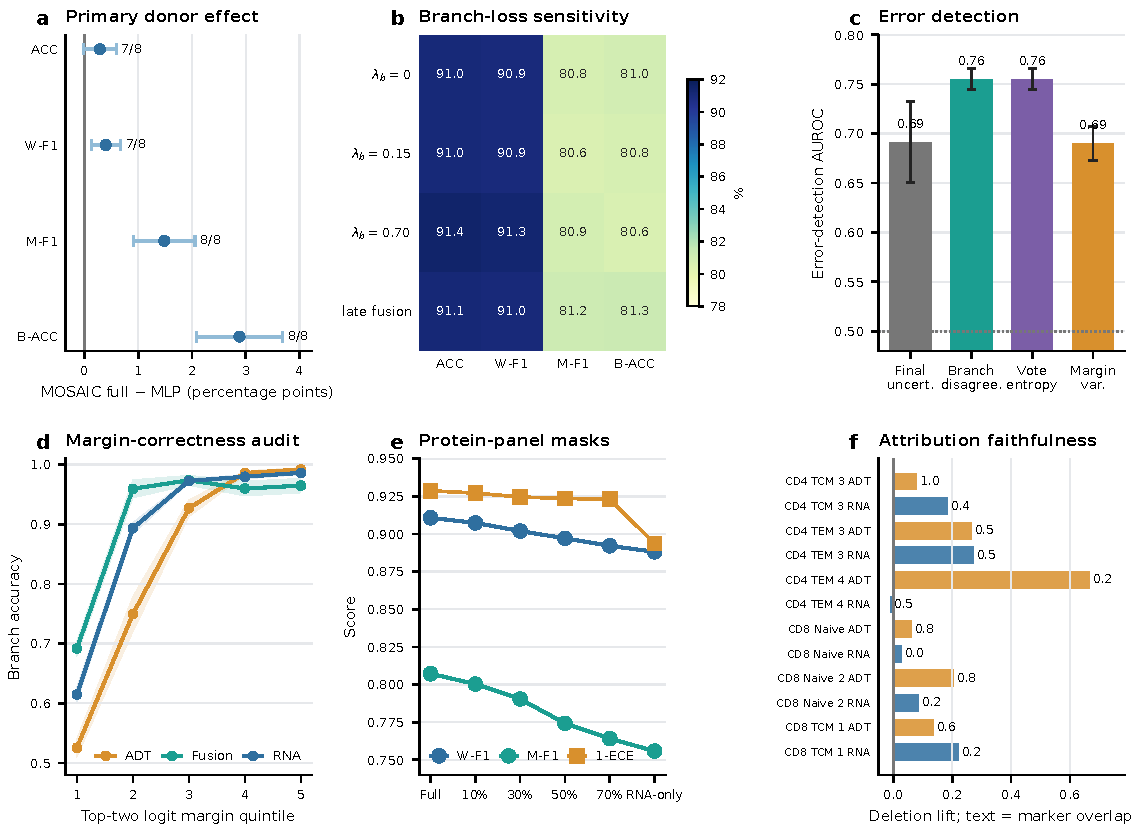
\includegraphics[width=0.94\textwidth]{Fig/Fig2_MOSAIC_V36_evidence.pdf}
\caption{\textbf{Donor-disjoint performance and mechanism evidence.} (a) Donor-paired MOSAIC full minus MLP differences with 95\% intervals and positive-donor counts. (b) Retrained branch-loss sensitivity under the primary nested donor protocol. (c) Error-detection AUROC for final uncertainty and branch-derived audit scores. (d) Branch accuracy across top-two logit-margin quintiles for RNA, ADT and fusion branches. (e) W-F1, M-F1 and calibration retention under deterministic protein-panel masks. (f) Attribution faithfulness by top-feature deletion lift; text values show canonical-marker overlap fractions.}
\label{fig:evidence}
\end{figure*}

\section{Discussion}

The primary result is a donor-disjoint, leakage-controlled evaluation of fine-grained multimodal annotation. MOSAIC improved W-F1 and M-F1 over a matched early-fusion MLP across donors, while the ACC interval crossed zero. This distinction matters for fine immune annotation: rare and sibling labels contribute little to overall accuracy but strongly affect macro-level and balanced metrics. Protein masking showed that a full-input model can degrade gradually, but rare-class performance and calibration remain sensitive when the ADT panel disappears. Leave-class-out rejection was useful for some targets and weak for others, and the B naive lambda failure illustrates how unknown detection can fail when a fine boundary lacks a matched protein marker.

The main contribution is the evaluation framing. MOSAIC specifies a deployment setting--donor-disjoint fine-level CITE-seq annotation--and tests adjacent risks that affect reference reuse: module failure, missing-panel degradation, target-dependent rejection and attribution faithfulness. The architecture should be interpreted similarly narrowly. Branch supervision exposes modality-specific competence, and HSR restricts local correction to declared sibling labels, but no-HSR, no-KD and uniform fusion performed as well as or better than full for some metrics. Higher branch supervision improved ACC/W-F1 in the sensitivity matrix, whereas late-fusion-only training gave the best M-F1 and balanced accuracy. The recommended default is therefore MOSAIC full when audit outputs are required, with uniform fusion documented as a closed-set sensitivity option rather than a new post hoc default.

MMoCHi remained superior on its native sorted hierarchy. This is consistent with a marker-defined method being effective in a small, structured label space. MOSAIC addresses high-dimensional reference classification, but that distinction does not erase the negative comparison. Similarly, canonical-marker enrichment supports biological concordance for selected labels, not discovery of causal biomarkers. These results place MOSAIC between two extremes: it is more inspectable than a monolithic early-fusion classifier, but it is not a substitute for a carefully curated marker hierarchy when that hierarchy matches the task.

Limitations include only eight PBMC donors, one compatible direct hierarchy baseline, complete training-label support in natural donor folds, and post hoc masking rather than mask-aware training. Leave-class-out targets are constructed pseudo-unknowns, PDC101 uncertainty modes are not interchangeable, and donor-pair attribution statistics are descriptive because pairs overlap. The older random-cell, patient-disjoint COVID-19 \citep{stephenson2021}, 5P assay-cohort and COMBAT analyses are retained in the Supplement as secondary breadth evidence and are not pooled with the primary donor-level inference.

Future work should focus on the modules that were not validated here. A panel-aware training objective could replace post hoc masking and explicitly teach RNA-only or partial-ADT fallback. HSR should be redesigned with validation-selected activation policies or hierarchy-aware loss terms that prove benefit before test evaluation. Unknown handling should move from leave-class-out stress tests to prospective external datasets with true absent or novel states. Finally, attribution evidence should be extended beyond the selected sibling classes to full deletion/insertion curves across more labels.

In summary, MOSAIC provides a reproducible framework for fine-grained RNA--ADT annotation with explicit modality branches, bounded local intervention and audit outputs. Nested donor evaluation supports W-F1 and M-F1 gains over matched early fusion, while direct ablations delimit rather than validate HSR, KD and gating. Missing-panel, pseudo-unknown, PDC101 and attribution analyses define where the current model is reliable and where additional work is required.

\section{Data availability}

PBMC 3P and 5P data are from GEO accession GSE164378. The COVID-19 cohort is from ArrayExpress E-MTAB-10026. PDC101 is from GEO GSE229791. COMBAT is available through Human Cell Atlas project \texttt{cdabcf0b-7602-4abf-9afb-3b410e545703}, EGA study EGAS00001005493 and Zenodo DOI 10.5281/zenodo.6120249 \citep{combat2022}. Processed split manifests and source-record checks are included with the reproducibility artifacts described in the Supplementary Material.

\section{Code availability}

Source code, configuration files, split manifests, compact evidence tables, tests, environment metadata and checksum records are available under the MIT License at \url{https://github.com/printfnice/MOSAIC}. Raw participant data, cached matrices and model checkpoints are not distributed through the GitHub repository. Pretrained checkpoints and an archival DOI can be added through a stable external archive before formal journal submission if required.

\section{Funding}

No specific funding was received for this work.

\section{Author contributions}

Hai Yang and Linhao Wu conceived the study. Linhao Wu led the implementation, data processing, experiment execution, result auditing, visualization and manuscript drafting. Hai Yang contributed to method design, experiment planning, interpretation and manuscript drafting. Dan Zhou and Tianyi Zhou contributed to study discussion, biological interpretation and manuscript review. Qin Zhou, Ting Xiao, Qian Zhang and Jing Zhang contributed to data interpretation and manuscript review. Zhe Wang supervised the study and revised the manuscript.

\section{Conflict of interest}

The authors declare no competing interests.

\section{Acknowledgements and use of AI-assisted tools}

AI-assisted tools were used for code assistance, artifact auditing, table generation and language editing. All analyses, figures, citations and conclusions were designed, verified and are the responsibility of the human authors.

{\footnotesize
\setlength{\bibsep}{0pt}
\bibliographystyle{oup-plain}
\bibliography{references}
}

\end{document}
